\documentclass[unicode,hyperref={unicode=true},aspectratio=169]{beamer}
\mode<presentation>
{
  \usecolortheme[RGB={55,109,160}]{structure}
  \usetheme{Dresden}
  \setbeamertemplate{navigation symbols}{}
  \setbeamertemplate{blocks}[rounded][shadow=true]
  \setbeamertemplate{items}[ball]
  \setbeamercovered{invisible}
}

\defbeamertemplate*{footline}{infolines theme}
{
  \leavevmode%
  \hbox{%
  \begin{beamercolorbox}[wd=\paperwidth,ht=2.25ex,dp=1ex,right]{date in head/foot}%
    \insertframenumber{} / \inserttotalframenumber\hspace*{2ex}
  \end{beamercolorbox}}%
  \vskip0pt%
}

\setbeamertemplate{headline}{
	\begin{beamercolorbox}[wd=\paperwidth,ht=3.25ex,dp=1ex,left]{date in head/foot}
		~~\insertsection
	\end{beamercolorbox}
}

\setbeamerfont{section title}{parent=title}
\setbeamercolor{section title}{parent=titlelike}
\defbeamertemplate*{section page kb}{default}[1][]
{
  \centering
	\begin{beamercolorbox}[sep=8pt,center,#1]{section title}
	  \usebeamerfont{section title}\insertsection\par
	\end{beamercolorbox}
}
\newcommand*{\sectionpagekb}{\usebeamertemplate*{section page kb}}
\setbeamercolor{block title}{use=structure,fg=white,bg=structure.fg!75!black}

\usepackage{etex}
\usepackage[T1]{fontenc}
\usepackage[utf8]{inputenc}
\usepackage[russian]{babel}
\usepackage{graphicx}
\usepackage{fancyvrb}
\usepackage{shortvrb}
\usepackage{amsthm}
\usepackage[]{url}
%\MakeShortVerb{!}
\usepackage{listings}
\lstset{ %
    stringstyle=\color{red},
    extendedchars=\true,
    inputencoding=utf8,
    columns=fixed,keepspaces
}
\usepackage{enumerate}
\usepackage{tikz}
\usepackage{xy}
\usepackage{algorithm}
\usepackage{algorithmicx}
\usepackage{algpseudocode}
\usepackage{latexsym}
\usepackage{subfig}
\usepackage{tikz}
\usepackage{dirtree}
\usetikzlibrary{positioning,arrows}

\title[]
{Automation of device and machine development for QEMU*}

\author[]{\textbf{%
Vasiliy Efimov \texttt{<real@ispras.ru>} (corresponding)}\\%
Aleksandr Bezzubikov \texttt{<abezzubikov@ispras.ru>}\\%
Danila Bogomolov \texttt{<bda@ispras.ru>}\\%
Oleg Goremykin \texttt{<goremykin@ispras.ru>}\\%
Vartan Padaryan \texttt{<vartan@ispras.ru>}%
}

\institute[]{Ivannikov Institute for System Programming of the RAS}

\date[]{2017 Ivannikov ISPRAS Open Conference, Moscow, \(1^{st}\) December\\%
\vfill
\textit{\tiny *This work is supported by RFBR, grant No 16-29-09632}}

\begin{document}

\begin{frame}
\titlepage
\end{frame}



\begin{frame}[fragile]{The problem}
%\item Чтобы задействовать все возможности динамического анализа нужен эмулятор с
%поддержкой соответствующей вычислительной машины.
%В данном случае используется эмулятор QEMU.
%\vfill
Development of either device or machine model for QEMU is a
time-consuming task. Therefore, an automation is required.
\vfill
\begin{center}
\begin{tabular}{l|c|c|c|c|c}
Emulator/  & \multicolumn{2}{c|}{Machine}   & \multicolumn{2}{c|}{Device development} & Debug \\
Simulator  & \multicolumn{2}{c|}{composing} & \multicolumn{2}{c|}{automation}         & Tools \\
           & GUI & API                      & GUI & API                               &       \\
\hline
Simics     &  +  & C++, Python              & .   & DML \(\rightarrow\) C++           & .     \\
AMD SimNow &  +  & C++                      & .   & .                                 & .     \\
gem5       &  .  & C++, Python              & .   & .                                 & .     \\
OVPSim     &  .  & C, TCL \(\rightarrow\) C & .   & TCL \(\rightarrow\) C             & +     \\
QEMU       &  +  & C, CLI                   & .   & .                                 & .     \\
\end{tabular}
\end{center}
\end{frame}



\begin{frame}{The goal}
The goal is to automate the development of both device and machine for QEMU
emulator.

\vfill

{Objectives}
\begin{itemize}
\item analyse QEMU internals
\item search the workflow for stages to automate
\item develop a toolset automation
\item evaluate the toolset
\end{itemize}
\end{frame}



\section{Automation concepts}
\begin{frame}
\sectionpagekb
\begin{itemize}
\item Classic development workflow
\item QEMU Object Model (QOM)
\item Device modelling API
\item Machine composition API
\item Proposed workflow
\end{itemize}
\end{frame}



\begin{frame}{Classic development workflow}
\begin{center}
\includegraphics[height=0.8\textheight]{workflow-old-en.png}
\end{center}
\end{frame}



\section{Automation concepts}
\begin{frame}{QEMU Object Model (QOM)}
\begin{minipage}{0.49\textwidth}
\dirtree{%
.1 object .
    .2 machine .
    .2 device .
        .3 sys-bus-device .
            .4 device .
        .3 pci-device .
        .3 cpu, {...} .
    .2 bus .
        .3 PCI .
            .4 PCIE .
        .3 System .
        .3 usb-bus, {...}.
    .2 irq .
    .2 qemu:memory-region .
}
\hfill
\end{minipage}
\hfill
\begin{minipage}{0.49\textwidth}
\begin{itemize}
\item OOP in C (like Gnome library`s gobject)
\item Hierarchy node is called a \textit{type}
\item type =~\textit{class} +~\textit{instance}
\item class/instance =~\textit{structure}~(\texttt{struct},~C)
+~\textit{constructor}~(a callback, C)
\item \texttt{object} is a type that supports \textit{properties} to
both class and instance.
\item a property is an opaque value identified by a \textit{string} and
accessed through \texttt{set} and \texttt{get} function.
\end{itemize}
\end{minipage}
\end{frame}



\begin{frame}{Device modelling API}
\includegraphics[height=0.7\textheight]{device-model-ex-en.png}
\vfill
\textit{Interface code} is composed using finite set of API elements. Each the
element has finite set of parameters. Given those parameters, a draft with
interface code stubs can be generated for a device.
\end{frame}



\begin{frame}[fragile]{Machine composition API (example)}
\lstset{language=C}
\begin{lstlisting}
/* device instance creation */
dev = qdev_create(parent_bus, QOM_TYPE_NAME);

/* specification of properties */
object_property_set_TYPE(dev, PROP_VALUE, PROP_NAME, ...);

/* device instance "realization" */
qdev_init_nofail(dev);

/* mapping of registers */
sysbus_mmio_map(dev, REG_INDEX, REG_ADDRESS);

/* interrupt lines binding */
my_incoming_irq = qdev_get_gpio_in(dev, IN_IRQ_INDEX);
sysbus_connect_irq(dev, OUT_IRQ_INDEX, neighbour_incoming_irq);
\end{lstlisting}
\end{frame}



\begin{frame}{Machine composition API specifics}

\begin{itemize}
\item Machine content is described in a declarative way.
\item An object model is used for content description.
\item A complicated device interconnection is difficult to sense in form of
code.
\end{itemize}

\begin{center}
Therefore, the graphical editor was implemented. It represent a machine in
a schematic form. The editor generates a code for the machine draft.
\end{center}

\end{frame}



\begin{frame}{Proposed workflow}
\begin{center}
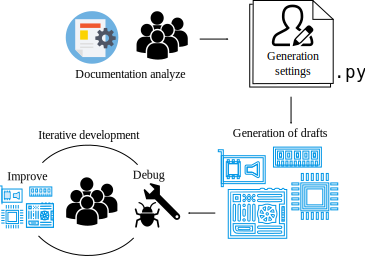
\includegraphics[height=0.8\textheight]{workflow-en.png}
\end{center}
\end{frame}



\section{Developed toolset}
\begin{frame}{}
\sectionpagekb
\begin{itemize}
\item Toolset infrastructure
\item Settings format
\item Generator capabilities
\item Examples
\item GUI
\item Existing QEMU code feedback
\end{itemize}
\end{frame}{}



\begin{frame}{}
\begin{center}
\includegraphics[height=0.98\textheight]{main-en.png}
\end{center}
\end{frame}



\begin{frame}{Device draft generation capabilities}
\begin{center}
\begin{tabular}{l|r}
Device class & Capabilities \\
\hline
Any          & QOM registration \\
             & VM state and property declaration \\
             & timers \\
             & character and block devices \\
             & network interface \\
\hline
System       & MMIO \\
bus          & PMIO \\
device       & in/out IRQ \\
\hline
PCI(E)       & BAR \\
device       & out IRQ (INTx) \\
function     & MSI(X) \\
             & identification information
\end{tabular}
\end{center}
\end{frame}



\begin{frame}[fragile]{Fast Ethernet adapter draft generation settings example}
\lstset{language=Python}
\begin{lstlisting}
obj55 = PCIExpressDeviceDescription(
    name = "AM79C971",    # model name
    vendor = "0x1022", device = "0x2000", pci_class = "0x0200",
    revision = 0x1,
#   subsys = None, subsys_vendor = None,
    directory = "net",    # directory name
    irq_num = 0x1,
    mem_bar_num = 0x1,
    nic_num = 0x1,
    timer_num = 0x1,
#   msi_messages_num = 0,
#   char_num = 0,
#   block_num = 0
)
\end{lstlisting}
\end{frame}

\begin{frame}
\begin{center}
\includegraphics[height=0.9\textheight]{AM79C971.jpg}
\end{center}
\end{frame}



\begin{frame}[fragile]{Machine content description}

\begin{minipage}{0.61\textwidth}
\dirtree{%
.1 Node .
    .2 BusNode .
        .3 SystemBusNode .
        .3 PCIExpressBusNode .
        .3 [ISA, IDE, I2C]BusNode .
    .2 DeviceNode .
        .3 SystemBusDeviceNode .
        .3 PCIExpressDeviceNode .
    .2 IRQLine .
    .2 IRQHub .
    .2 MemoryNode .
        .3 MemoryLeafNode .
            .4 MemoryAliasNode .
            .4 MemoryRAMNode .
            .4 MemoryROMNode .
}
\end{minipage}
\begin{minipage}{0.37\textwidth}
This type hierarchy is based on QOM. \\
\vfill
\texttt{IRQHub} allows to deliver one IRQ to many devices. \\
\vfill
Most part of memory address space is defined by devices internally.
But several kinds of memory (like a RAM or a simple ROM) have to be defined
explicitly.
\texttt{MemoryNode} ancestors are used for it. \\
\end{minipage}
\end{frame}



\begin{frame}
\begin{center}
\includegraphics[height=0.98\textheight]{REMOTE.jpg}
\end{center}
\end{frame}



\begin{frame}{Bus interconnection example in GUI}
\begin{center}
\includegraphics[width=0.7\linewidth]{bus_widget.jpg}
\end{center}
\end{frame}



\begin{frame}{IRQ line interconnection example in GUI}
\begin{center}
\includegraphics[height=0.8\textheight]{irq_widget.jpg}
\end{center}
\end{frame}



\begin{frame}{Existing QEMU code feedback}
\begin{minipage}{0.35\textwidth}
\includegraphics[height=0.8\textheight]{heuristics-en.png}
\end{minipage}
\hfill
\begin{minipage}{0.63\textwidth}
\begin{itemize}
\item Automatic header analysis
    \begin{itemize}
    \item Inclusion graph (used to generate header inclusions)
    \item Preprocessor macros (used by both GUI and generator core)
    \end{itemize}
\item Heuristic based support for different QEMU version.
    \begin{itemize}
    \item A new value is propagated towards future commits.
    \item An old value is propagated:
        \begin{enumerate}
        \item towards past commits,
        \item towards future commits.
        \end{enumerate}
    \item During merging new values are chosen.
    \item Given SHA1, the actual value can be obtained.
    \end{itemize}
\end{itemize}
\end{minipage}
\end{frame}



\section{The toolset usage examples}
\begin{frame}
\sectionpagekb
\begin{itemize}
\item Intel Q35 chipset based PC
\item СISCO 2600 series router (C2621XM)
\end{itemize}
\end{frame}



\begin{frame}{Intel Q35 chipset based PC}
\begin{itemize}
\item There is another implementation in QEMU already. It is one of most
complicated machines in the emulator.
\item The goal of this experiment is to prove the proposed workflow correctness.
\item All requred devices are already present in QEMU.
\item Several old devices were updated using the toolset.
\end{itemize}
\end{frame}



\begin{frame}{Q35 machine scheme}
\begin{center}
\includegraphics[height=0.9\textheight]{Q35-h.png}
\end{center}
\end{frame}



\begin{frame}{Evaluation*}
\begin{center}
\begin{tabular}{l|lll}
Stage          & Files     & Lines     & Lines   \\
               & touched   & inserted  & deleted \\
\hline
Preparation**  & 4         & 42        & 31      \\
Generation     & 8         & 599       & 0       \\
Implementation & 5         & 162       & 93***   \\
Total          & 12        & 803       & 31      \\
\end{tabular}
\end{center}
\vfill
\it{*The measurements were made using git diff.} \\
\it{**A refactoring mostly.}\\
\it{***Note that amount of deleted lines is a measure of piece of generated
code to be adjusted.}\\
\end{frame}



\begin{frame}{С2600 series router (C2621XM)}
\begin{itemize}
\item Based on Dynamips.
\item CPU PowerPC MPC860 presents in QEMU \textit{except for full system
emulation support}.
\item Both machine and devices were implemented using the toolset (except for
CPU).
\end{itemize}
\end{frame}



\begin{frame}{C2621XM router scheme}
\begin{center}
\includegraphics[height=0.9\textheight]{C2600.png}
\end{center}
\end{frame}



\begin{frame}{Evaluation}
\begin{center}
\begin{tabular}{l|lll}
Stage          & Files     & Lines     & Lines   \\
               & touched   & inserted  & deleted \\
\hline
Preparation*   & 8         & 128       & 35      \\
Generation     & 37        & 2186      & 0       \\
Implementation & 31        & 4747      & 419     \\
Total          & 45        & 6642      & 35      \\
\end{tabular}
\end{center}
\vfill
\it{*Memory management unit, CPU's special registers and interrupt support,
PCI identifiers.}
\end{frame}



\begin{frame}{Evaluation*}
\begin{center}
\begin{tabular}{l|ll}
Device            & Configuration size & Draft size \\
\hline
MPC860\_IC        & 6                  & 125           \\
C2600\_PCI\_HOST  & 6                  & 133           \\
C2600\_PCI        & 7                  & 82            \\
NS16552           & 7                  & 181           \\
C2600\_IO\_FPGA   & 8                  & 137           \\
CISCO\_REMOTE     & 7                  & 152           \\
AM79C971          & 12                 & 175           \\
\end{tabular}
\end{center}
\vfill
\it{*The size is measured in lines.}
\end{frame}



\section{Conclusion}
\begin{frame}
\sectionpagekb
\begin{itemize}
\item Results
\item Future work
\end{itemize}
\end{frame}



\begin{frame}{Results}
\begin{itemize}
\item The first stage of device and machine model development was automated
using the code draft generation toolset.
\item A generation configuration is written in Python.
\item The size of resulting device draft is 11-25 times bigger than size of
corresponding configuration.
\item The GUI was implemented including schematic machine editor.
\item The toolset supports complex machines like Intel Q35.
\item The piece of generated code is between \(1/4\) and \(3/4\) depending on
amount of available device models.
\item Existing QEMU code is accounted including QEMU version adaptation
mechanism.
\end{itemize}
\end{frame}



\begin{frame}{Future work}
Runtime debug feedback form QEMU.
\vfill
\begin{center}
\includegraphics[height=0.8\textheight]{gdb-feedback-en.png}
\end{center}
\end{frame}



\section{The End}
\begin{frame}{}
\begin{center}
\vfill
\sectionpagekb
\vfill
Thank you for your attention!
\vfill
Questions?
\vfill
\end{center}
\end{frame}



\end{document}
